\documentclass[10pt]{beamer}
\usetheme{Antibes}

\usepackage{graphicx}
\graphicspath{{../figures/}}


\title{Gendered Pronoun Resolution}
\author[Dhruv, Prateek]{ Dhruv Patel (14528) \and Prateek Sachan (15754)}
\institute[CSA, IISc.]{Computer Science and Automation, Indian Institute of Science}
\begin{document}
\begin{frame}
  \maketitle
\end{frame}

\section{Problem Introduction}
\begin{frame}{Problem}
  \begin{itemize}
  \item<+-> We are given a sentence or sentences, two candidate nouns within a sentence and a pronoun
  \item<+-> Task is to identify which of these two candidates refers to that pronoun
  \end{itemize}

  \begin{block}<+->{Example}
    Impressed by her beauty, her warrior skills, and the fact that she was able to locate him, she is promoted to a position similar to that later held by her half-sister, Talia. As a right hand associate, she accompanies him during his adventures. Ra's is so impressed with her abilities, he even allows Nyssa to use his Lazarus Pits. Like \textit{\textbf{her}} sister \textbf{Talia}, \textbf{\underline{Nyssa}} eventually becomes disenchanted with Ra's genocidal plans to ``cleanse the Earth'', and disassociates herself from her father sometime in the early 20th century.
  \end{block}
  \begin{itemize}
  \item<+-> Introduced as Kaggle competition by Google AI
  \end{itemize}

\end{frame}

\section{Datasets}
\begin{frame}{Datasets}
  \pause
  \begin{block}<+->{GAP Webster et al. (2018)\cite{webster2018gap}}
    \begin{itemize}
    \item<+-> Balanced Dataset
    \item<+-> 2000 Development, 2000 Test and 454 validation sentences
    \end{itemize}

    \begin{quote}<+->
      \textbf{\underline{Kathleen}} first appears when \textbf{Theresa} visits \textbf{\textit{her}} in a prison in London.
    \end{quote}
  \end{block}

  \begin{block}<+->{Definite Pronoun Resolution, Rahman et al. (2012), \cite{rahman2012resolving}}
    \begin{itemize}
    \item<+-> Unbalanced dataset
    \item<+-> 1886 sentences in total (943 sentence pairs) (When used, we used all for training)
    \end{itemize}

    \begin{quote}<+->
       James asked \textbf{Robert} for a favor, but \textit{\textbf{he}} refused.

       \textbf{James} asked Robert for a favor, but \textit{\textbf{he}} was refused.
      
    \end{quote}
  \end{block}

\end{frame}

\subsection{Data Augmentation}
\begin{frame}{Data Augmentation}
  \begin{itemize}
  \item<+-> 2000 sentences, two less data to train.
  \item<+-> Our models quickly overfitted. We were unable to pass our own baseline.
  \end{itemize}
  \begin{block}<+->{Hypothesis}
    To neural network, if only ``Jon Snow doesn't know anything'' is given, the effect should be similar to when ``John Wick doesn't know anything'' is given instead.
  \end{block}
  
  \uncover<+->{So we replace all occurrences of Jon with John and of Snow with Wick. There could be same occurrence for different \textbf{unrelated} objects by chance. We assume that, that doesn't happen often.}

  \uncover<+->{As a side effect Ramsey Snow will become Ramsey Wick. In most cases this is not a problem. }

\end{frame}

\begin{frame}{Method}
  \begin{itemize}
  \item If both candidate A and candidate B has less than four words and neither of them contains characters from ``,(*)''
    \begin{itemize}
    \item If pronoun is \textbf{he}, \textbf{him} or \textbf{his}
      \begin{itemize}
      \item Find alternative male candidate of same length as A, such that no word of old A or old B is contained in new proposal.
      \item Find alternative male candidate of same length as B, such that no word of old A or old B is contained in new proposal.
      \end{itemize}
    \end{itemize}
    \begin{itemize}
    \item If pronoun is \textbf{she}, \textbf{her} or \textbf{hers}
      \begin{itemize}
      \item Find alternative female candidate of same length as A, such that no word of old A or old B is contained in new proposal.
      \item Find alternative female candidate of same length as B, such that no word of old A or old B is contained in new proposal.
      \end{itemize}
    \end{itemize}
  \item if old A and old B had any common word, modify proposals to behave similarly to old candidates.
  \item replace old A with new A, replace old B with new B.
  \end{itemize}
\end{frame}

\begin{frame}{Example}
  \begin{itemize}
  \item Tony Markham, a high school senior and the ``Tall Dark Stranger'' \underline{Betsy} fell in love with as a freshman, who has since become a good friend not only to \underline{Betsy} but the entire \underline{Ray} family. \underline{Mrs. Ray}, \underline{Betsy}'s mother. \underline{Mr. Ray}, \underline{Betsy}'s father, who owns a shoestore. \textbf{\underline{Margaret Ray}}, \textbf{\underline{Betsy}}'s sister who is five years younger than she is.

  \item Tony Markham, a high school senior and the ``Tall Dark Stranger'' \underline{Alyssa} fell in love with as a freshman, who has since become a good friend not only to \underline{Alyssa} but the entire \underline{Jolie} family. \underline{Mrs. Jolie}, \underline{Alyssa}'s mother. \underline{Mr. Jolie}, \underline{Alyssa}'s father, who owns a shoestore. \underline{Angelina Jolie}, \underline{Alyssa}'s sister who is five years younger than she is.
    
  \item Tony Markham, a high school senior and the ``Tall Dark Stranger'' \underline{Booth} fell in love with as a freshman, who has since become a good friend not only to \underline{Booth} but the entire \underline{Delgado} family. \underline{Mrs. Delgado}, \underline{Booth}'s mother. \underline{Mr. Delgado}, \underline{Booth}'s father, who owns a shoestore. \underline{Pam Delgado}, \underline{Booth}'s sister who is five years younger than she is.
  \end{itemize}    
\end{frame}

\begin{frame}
  \begin{figure}
    \centering
    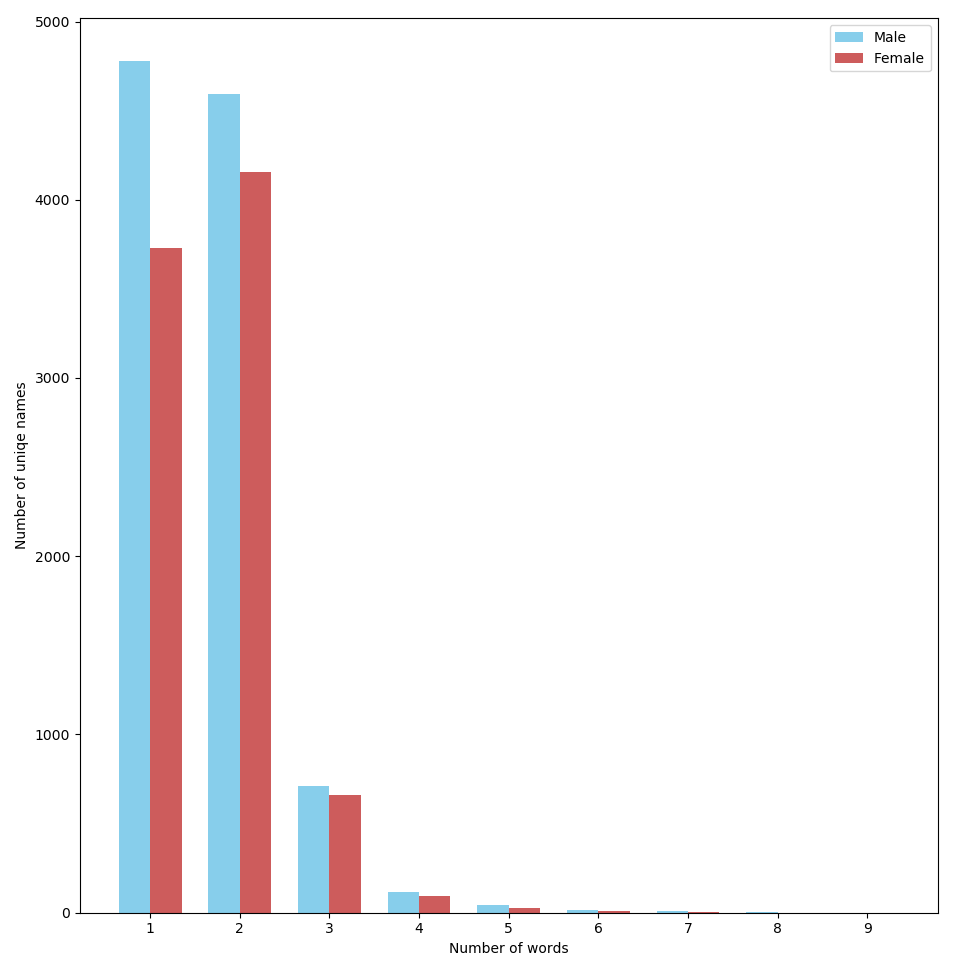
\includegraphics[width=.7\textwidth]{augment_dist.png}
    \caption{Distribution of names}
    \label{fig:dist_names}
  \end{figure}
\end{frame}

\subsection{Metrics}
\begin{frame}{Metrics}
To compare our results with baseline proposed by Webster et al.\cite{webster2018gap}, we use micro average of F1-scores. To compare our results with other Kaggle competitors, we used cross entropy loss $\mathcal{L}$.

\[
  \mathcal{L} = - \frac{1}{N} \sum_{i=1}^N \sum_{j \in \{A, B, N\}} (y_i^j* log(\sigma(\hat{y_i^j}))).
\]

Where $y_i^j$ is 1 if $j$ is correct candidate for $i^{th}$ example. N denotes neither case. $\hat{y_i^j}$ denotes predicted probability for class $j$ for $i^{th}$ example.
\end{frame}

\section{Method}
\begin{frame}{Method}
  \begin{itemize}
  \item<+->  Earlier we started with ambitious goal. We chose all candidates using Named Entity Recognition.
    \begin{itemize}
    \item<+-> Class imbalance
    \item<+-> Models didn't perform well. So we used simpler setting.
    \end{itemize}

  \item<+->We adapted Lee et al's architecture \cite{lee2017end}.
    \begin{itemize}
    \item<+-> No need for mention scoring.
    \item<+-> Different scoring functions were tried. Best we found was three layer fully connected network.
    \end{itemize}
  \end{itemize}
\end{frame}
\begin{frame}{Architecture}
  \begin{figure}
    \centering
    \includegraphics<+>[width=.8\textwidth]{arch1.png}%
    \includegraphics<+>[width=.8\textwidth]{arch2.png}%
    \includegraphics<+>[width=.8\textwidth]{arch3.png}%
    \includegraphics<+>[width=.8\textwidth]{arch4.png}
    \caption{Architecture}
    \label{fig:arch}
  \end{figure}
\end{frame}

\section{Experiments}
\begin{frame}{Experiments}
  \begin{itemize}
  \item<+-> Different layers of BERT large and base model were tried.
  \item<+-> With and without DPR dataset
  \item<+-> Scoring function used three linear layers of size 62, 32, and 1 respectively with ReLU activations.
  \item<+-> Also tried LSTM with single layer of 256 units between BERT and scoring function.
  \item<+-> To combine different tokens of A and B, we tried attention mechanism and simple mean method.
  \item<+-> Best results were obtained without RNN, with weight decay of 0.001 and dropout of 0.5. Adam optimization was used.
  \end{itemize}
\end{frame}

\section{Results}
\begin{frame}{Baselines}
  \begin{block}<+->{From Webster et al. \cite{webster2018gap}}
    \begin{table}
      \centering
      \begin{tabular}{|l|r|r|r|}
        \hline
        & M & F & O \\
        \hline
        Wiseman et al. \cite{wiseman2016learning} & 68.4 & 59.9 & 64.2 \\
        Lee et al. \cite{lee2017end} & 67.2 & 62.2 & 64.7 \\
        \hline
      \end{tabular}
    \end{table}

    \uncover<+->{However not trained on GAP dataset. Lee et al. was trained on Onto Notes.}
  \end{block}
  
  \begin{block}<+->{Ours}
    An SVM trained on the output of 8th layer BERT base. (input to SVM was 768*3 dimensional vector)
    \begin{table}
      \centering
      \begin{tabular}{|l|r|r|r|}
        \hline
        & M & F & O \\
        \hline
        SVM-8 & \textbf{77.10} & \textbf{79.10} & \textbf{78.10} \\
        \hline
      \end{tabular}
    \end{table}
  \end{block}
\end{frame}

\begin{frame}{Stage 1}
  \begin{table}
    \centering
    \begin{tabular}{|l|r|r|r|}
      \hline
      & M & F & O \\
      \hline
      SVM-8 & 77.10 & 79.10 & 78.10 \\
      \hline
      MLP             & 89.10 &88.00 & 88.55 \\
      MLP-attn         &  89.50 & 88.40 & 88.95 \\
      MLP-dpr           & 88.90 & 88.70 & 88.80 \\
      MLP-dpr-attn    & 90.10 & 87.90 & 89.00 \\
      \hline
    \end{tabular}
    \caption{F1 score Results}
    \label{tab:f1}
  \end{table}

  \begin{table}
    \centering
    \begin{tabular}{|l|r|r|r|r|}
      \hline
      &M & F & O \\
      \hline
      SVM-8          & 0.5127 & 0.5077 & 0.5102 \\
      \hline
      MLP  & 0.2669 & 0.3412 & 0.3041 \\
      MLP-attn   & 0.2828 & 0.3252 & 0.3040 \\
      MLP-dpr      & 0.2752 & 0.3187 & 0.2969 \\
      MLP-dpr-attn & 0.2706 & 0.3367 & 0.3036 \\
      \hline
    \end{tabular}
    \caption{Cross Entropy Loss on stage 1 test set}
    \label{tab:ce1}
  \end{table}
\end{frame}

\begin{frame}{Stage 2} 
  \begin{table}
    \centering
    \begin{tabular}{|l|r|}
      \hline
      & O \\
      \hline
      SVM-8          &  0.7809 \\
      \hline
      RNN-MLP & 0.3529 \\
      \hline
      MLP  & 0.2462 \\
      MLP-attn   & 0.2545 \\
      MLP-dpr      & 0.2727 \\
      MLP-dpr-attn & 0.2517 \\
      \hline
      Kaggle First & 0.1366 \\
      Kaggle 25th & 0.2403 \\
      \hline
    \end{tabular}
    \caption{Cross Entropy Loss on stage 2 test set}
    \label{tab:ce2}
  \end{table}
\end{frame}

\begin{frame}
  \begin{table}
    \centering
    \begin{tabular}{|l|r|r|r|r|}
      \hline
      &    precision&    recall&  f1-score&    support \\
      \hline
      A&     0.8635&    0.9533&    0.9062&       856\\
      B&     0.9219&    0.8930&    0.9072&       925\\
      Neither&     0.8113&    0.5890&    0.6825&       219\\
      \hline
    \end{tabular}
    \caption{Precision-Recall of MLP}
    \label{tab:precisionrecall}
  \end{table}
\end{frame}

\section{Comments}
\begin{frame}{Comments}
  \begin{itemize}
  \item<+-> Lack of difference between attention mechanism and simple mean
    \only<+>{
      \begin{figure}
        \centering
        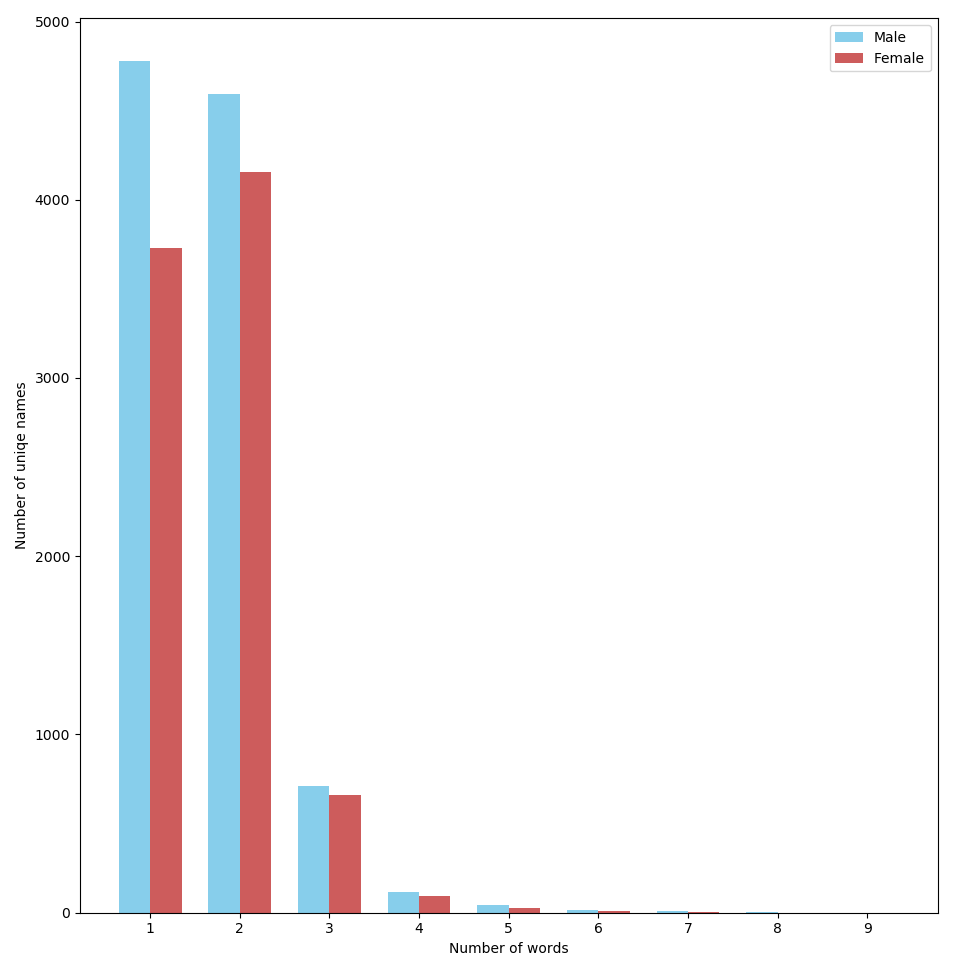
\includegraphics[width=.5\textwidth]{augment_dist.png}      
      \end{figure}
    }
  \item<+-> Bias
  \item<+-> Adaptability to more than two candidates
    \begin{figure}
      \centering
      \includegraphics<+>[width=.5\textwidth]{arch4.png}      
    \end{figure}
  \end{itemize}
\end{frame}

\section{}
\begin{frame}
  \centering
  \LARGE
  Thank You
\end{frame}
\begin{frame}
  \tiny
  \frametitle{References}
  \bibliographystyle{ieeetr}
  \bibliography{presentation.bib}
\end{frame}
\end{document}